\section{Progettazione}
\subsection{Use-Case Diagrams}
I tre attori principali che interagiscono con il sistema sono il Cliente (Customer), il Manutentore (Worker) e l'Amministratore (Admin).
Tutti gli attori derivano dalla classe \textbf{Utente} che espone i metodi per fare l'accesso ("Login") e registrarsi ("Sign-Up") al sistema.

Il \textbf{Customer} una volta autenticato, può acquistare articoli ("Buy item"), connettersi al distributore automatico ("Connect to Vending Machine") e ricaricare il proprio account ("Recharge account").

Il \textbf{Worker} può visualizzare i compiti assegnati ("View Assigned tasks"), visualizzare i dettagli dei compiti ("View task details") e segnalare il completamento di un compito ("Report task completion"). Inoltre, tramite il sistema può segnalare un problema alla Vending Machine.

L'\textbf{Admin} ha il ruolo con più funzionalità. L'Admin può gestire la creazione, lettura, aggiornamento, eliminazione degli utenti ("Manage Users CRUD"), che include "Add worker" (aggiungere manutentori), "Remove User" (rimuovere utenti) e "Update User Details" (aggiornare i dettagli degli utenti), oltre a "View/Search User" (visualizzare/cercare utenti).
Inoltre, l'Admin può gestire la creazione, lettura, aggiornamento, eliminazione dei distributori automatici ("Manage Vending Machines CRUD"), che comprende "Add Vending machine" (aggiungere distributori), "Remove Vending machine" (rimuovere distributori) e "Update Vending machine details" (aggiornare i dettagli dei distributori), e "View/Search Vending machine" (visualizzare/cercare distributori).
L'Admin è anche responsabile della gestione della creazione, lettura, aggiornamento, eliminazione degli articoli ("Manage Items CRUD"), potendo "Add item" (aggiungere articoli), "Remove item" (rimuovere articoli) e "Update item" (aggiornare articoli), oltre a "View/Search item" (visualizzare/cercare articoli). Infine, l'Admin ha accesso a "View sales analytics" (visualizzare le analisi delle vendite) e "View machine performance analytics" (visualizzare le analisi delle performance delle macchine).

È presente anche un attore "Vending Machine" che può eseguire auto-diagnostica ("Run Self-diagnostic"), mostrare articoli ("Display item"), accettare richieste di connessione ("Accept connection request") e segnalare lo stato della macchina o eventuali problemi ("Report Status/issue").

\begin{figure}
    \centering
    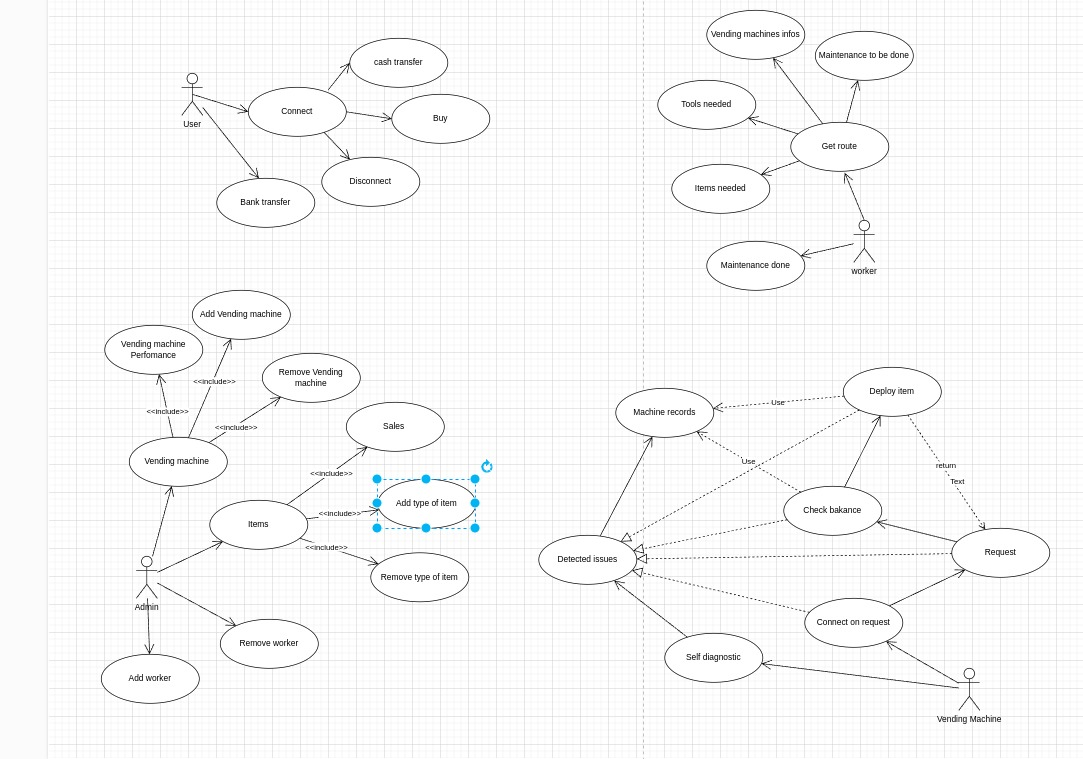
\includegraphics[width=0.5\linewidth]{assets/use-cases.jpeg}
    \caption{Use Cases}
    \label{fig:use cases}
\end{figure}

\subsection{Use-Case Templates}
Si descrivono nel dettaglio alcuni dei casi d'uso più importanti, suddivisi per attore. È sottointesa la precondizione di Login prima di qualsiasi operazione sul gestionale.

\subsubsection{Casi d'Uso del Customer}

\begin{table}[H]
\centering
\begin{tabularx}{\textwidth}{|p{2.5cm}|X|}
\hline
\textbf{UC-1} & \textbf{Buy Item} \\
\hline
\textbf{Description} & L'utente di tipo Customer acquista un prodotto da un distributore automatico a cui è connesso. \\
\hline
\textbf{Level} & User Goal \\
\hline
\textbf{Main Actors} & Customer \\
\hline
\textbf{Basic Course} &
\begin{enumerate}
    \item Il Customer si connette a un distributore automatico tramite l'applicazione mobile.
    \item Il sistema mostra gli articoli disponibili e il loro prezzo.
    \item Il Customer seleziona l'articolo desiderato.
    \item Il sistema verifica la disponibilità dell'articolo nell'inventario del distributore  e il saldo del Customer.
    \item Se l'articolo è disponibile e il saldo è sufficiente, il sistema eroga l'articolo.
    \item Il sistema aggiorna l'inventario del distributore e il saldo del Customer.
\end{enumerate} \\
\hline
\textbf{Alternative Paths} &
\begin{itemize}
    \item \textbf{4a. Saldo insufficiente:} Se il saldo del Customer non è sufficiente per l'acquisto, il sistema informa il Customer e propone di ricaricare l'account. Il Customer può scegliere di ricaricare (UC-2) o annullare l'acquisto.
    \item \textbf{5a. Errore di erogazione:} Se si verifica un errore durante l'erogazione dell'articolo, il sistema informa il Customer e registra un log di errore per la macchina. Il saldo del Customer non viene addebitato.
\end{itemize} \\
\hline
\end{tabularx}
\end{table}

\subsubsection{Casi d'Uso del Worker}
\begin{table}[H]
\centering
\begin{tabularx}{\textwidth}{|p{2.5cm}|X|}
\hline
\textbf{UC-3} & \textbf{Report Task Completion} \\
\hline
\textbf{Description} & L'utente di tipo Worker segnala il completamento di un'attività di manutenzione o rifornimento. \\
\hline
\textbf{Level} & User Goal \\
\hline
\textbf{Main Actors} & Worker \\
\hline
\textbf{Basic Course} &
\begin{enumerate}
    \item Il Worker visualizza l'elenco dei compiti assegnati.
    \item Il Worker seleziona il compito che ha completato.
    \item Il Worker conferma il completamento e, se necessario, aggiunge note.
    \item Il sistema aggiorna lo stato del compito a "completato" nel log di manutenzione.
\end{enumerate} \\
\hline
\textbf{Alternative Paths} &
\begin{itemize}
    \item \textbf{3a. Difficoltà nel completamento:} Se il Worker riscontra difficoltà nel completare il compito, può indicare un aggiornamento dello stato a "in progress" o "pending" e aggiungere note per richiedere supporto o indicare la necessità di ulteriori interventi.
\end{itemize} \\
\hline
\end{tabularx}
\end{table}

\begin{table}[H]
\centering
\begin{tabularx}{\textwidth}{|p{2.5cm}|X|}
\hline
\textbf{UC-4} & \textbf{Report Status/Issue (from Worker to Vending Machine)} \\
\hline
\textbf{Description} & L'utente di tipo Worker segnala un problema o un guasto riscontrato su un distributore automatico. \\
\hline
\textbf{Level} & User Goal \\
\hline
\textbf{Main Actors} & Worker, Vending Machine \\
\hline
\textbf{Basic Course} &
\begin{enumerate}
    \item Il Worker identifica un problema o un guasto su un distributore.
    \item Il Worker accede alla funzionalità di segnalazione problemi.
    \item Il Worker descrive il problema (es. codice errore, messaggio) e, se possibile, indica il tipo di guasto.
    \item Il sistema registra il problema nel log di rilevamento manutenzione [cite: 2, 6] e, se necessario, genera un nuovo compito di manutenzione.
\end{enumerate} \\
\hline
\textbf{Alternative Paths} &
\begin{itemize}
    \item \textbf{4a. Problema duplicato:} Se il problema è già stato segnalato e un compito è già in corso, il sistema notifica il Worker e gli chiede se vuole comunque aggiungere una nota al problema esistente.
\end{itemize} \\
\hline
\end{tabularx}
\end{table}

\subsubsection{Casi d'Uso dell'Admin}

\begin{table}[H]
\centering
\begin{tabularx}{\textwidth}{|p{2.5cm}|X|}
\hline
\textbf{UC-5} & \textbf{Manage Users CRUD} \\
\hline
\textbf{Description} & L'utente di tipo Admin gestisce gli account degli utenti (Clienti, Worker, Admin). \\
\hline
\textbf{Level} & User Goal \\
\hline
\textbf{Main Actors} & Admin \\
\hline
\textbf{Basic Course} &
\begin{enumerate}
    \item L'Admin accede alla sezione di gestione utenti.
    \item L'Admin può visualizzare l'elenco degli utenti  e cercare un utente specifico.
    \item L'Admin può aggiungere un nuovo utente (es. un nuovo Worker).
    \item L'Admin può modificare i dettagli di un utente esistente (es. ruolo, informazioni personali).
    \item L'Admin può rimuovere un utente dal sistema.
\end{enumerate} \\
\hline
\textbf{Alternative Paths} &
\begin{itemize}
    \item \textbf{3a. Utente esistente:} Se si tenta di aggiungere un utente con un username o email già esistente, il sistema notifica l'Admin.
    \item \textbf{5a. Utente con dipendenze:} Se l'Admin tenta di rimuovere un utente con transazioni o compiti assegnati attivi, il sistema chiede conferma o blocca l'operazione fino alla risoluzione delle dipendenze.
\end{itemize} \\
\hline
\end{tabularx}
\end{table}

\begin{table}[H]
\centering
\begin{tabularx}{\textwidth}{|p{2.5cm}|X|}
\hline
\textbf{UC-6} & \textbf{View Sales Analytics} \\
\hline
\textbf{Description} & L'utente di tipo Admin visualizza statistiche e analisi sulle vendite dei prodotti. \\
\hline
\textbf{Level} & User Goal \\
\hline
\textbf{Main Actors} & Admin \\
\hline
\textbf{Basic Course} &
\begin{enumerate}
    \item L'Admin accede alla sezione di visualizzazione delle statistiche.
    \item Il sistema presenta dati aggregati sulle vendite, come i prodotti più venduti, le fasce orarie di maggiore affluenza, e le entrate totali.
    \item L'Admin può applicare filtri per periodo, distributore o prodotto.
\end{enumerate} \\
\hline
\textbf{Alternative Paths} &
\begin{itemize}
    \item \textbf{3a. Nessun dato disponibile:} Se per i filtri selezionati non ci sono dati di vendita, il sistema visualizza un messaggio appropriato.
\end{itemize} \\
\hline
\end{tabularx}
\end{table}

% TODO: add mockup if you want